

\begin{figure}
\caption{The layout of a GPU}
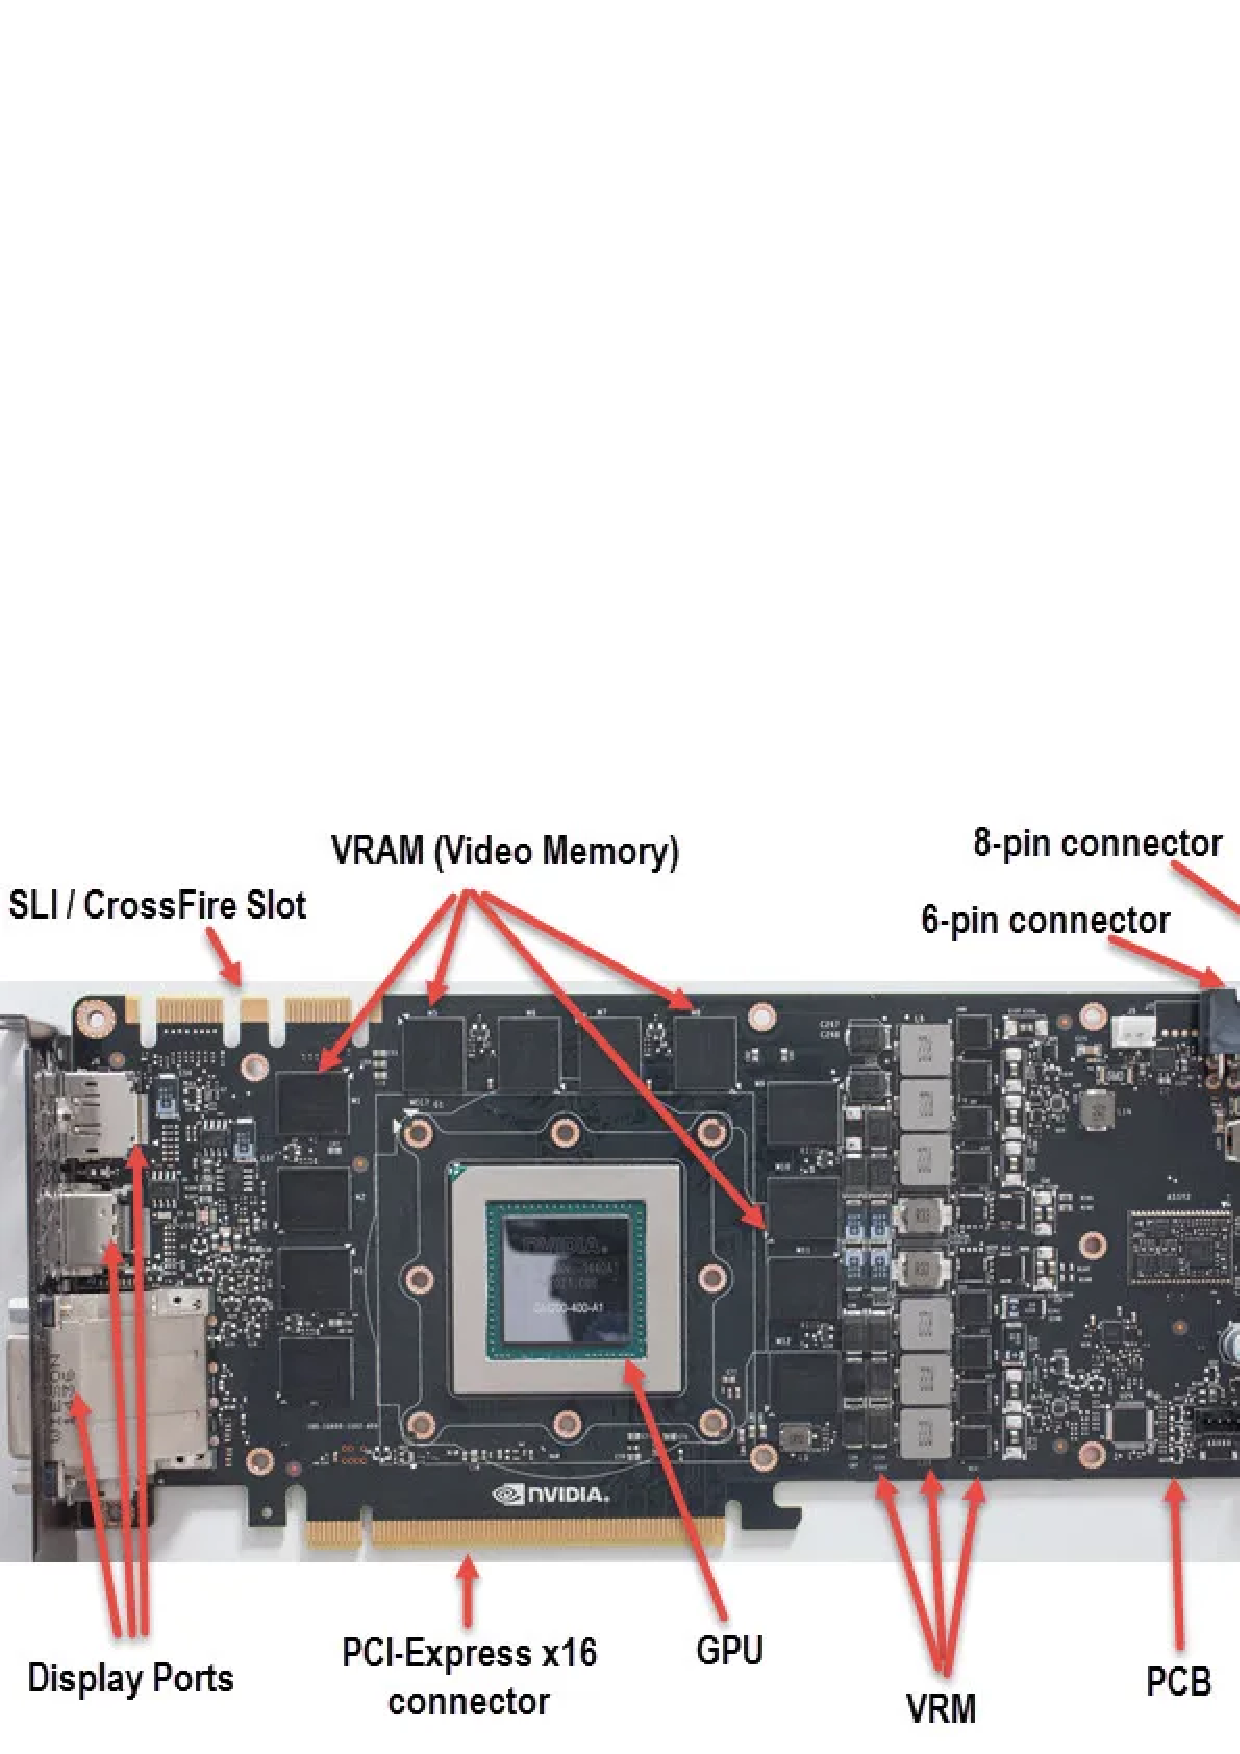
\includegraphics[width = \textwidth]{img/graphics-card-components-3119853491}
\end{figure}

\begin{figure}
\caption{Layout of a GPU chip}
\includegraphics[width = \textwidth]{img/pascal_gp104_block_diagram}
\end{figure}

\section{What do GPU's do?}
\label{sec:processor}
A GPU is used to process a 3D scene into an image which can be displayed to the screen. It gets the vertexes, materials, shaders and all other things which influence the look of a scene and turn it into an image, a frame. It does this 60 times per second most commonly, sometimes even faster if the screen is made for it and the GPU can handle that workload \cite{document1}. 
\\\\
The GPU consists of a couple things, see figure 1 for reference:
\begin{itemize}
	\item a PCIe slot
	\item GPU chip
	\item Display ports
	\item VRAM
	\item a PCB
	\item VRM
	\item x-Pin connectors
\end{itemize}
This list is not exhaustive. but will do for the purposes of explaining how a GPU works. Indeed, the GPU is both the name of the device and the chip on the device. This is due to the trivial name of the device being linked to the most important component. The GPU is a chip which has many smaller sub area's for parallel calculation as can be seen in figure 2, as a scene can contain a lot of objects, pixels and effects. Which can be somewhat calculated in parallel, keep in mind that on stage follows after another. Shaders are done after meshes for example, but multiple meshes can be calculated at the same time \cite{document1}. 
\\\\
The second most important component is VRAM. This is in essence just RAM but is located on the graphics card, which allows it to access this RAM quicker. This ram is used to store the input and output of the GPU. An example of what it would store is: information on the 3D scene and the partially completed image it is rendering. Where the amount of VRAM the card has will affect the complexity the scene may have before the card starts having issues with a bottleneck. 
\\\\
Just to not go on too long, The PCB is the plate all of the components are soldered on. The VRM regulates the voltage going to components, the display port outputs the frames the GPU calculates to a screen. The PCIe slot is where the GPU slots into the motherboard and where it communicates with the CPU. The x-pin connectors describes the amount of pins it needs, the more power a GPU needs the more pins it will require. These pins then connect back to the power supply in a desktop PC. 